\documentclass[11pt,a4paper]{article}

\usepackage[utf8]{inputenc}
\usepackage[T1]{fontenc}
\usepackage[spanish,english]{babel}
\usepackage{lmodern}
\usepackage{geometry}
\usepackage{microtype}
\usepackage{graphicx}
\usepackage{amsmath}
\usepackage{booktabs}
\usepackage{tabularx}
\usepackage{array}
\usepackage{longtable}
\usepackage{enumitem}
\usepackage{url}
\usepackage[hidelinks]{hyperref}
\usepackage{xcolor}
\usepackage{caption}
\usepackage{float}
\usepackage{fancyhdr}
\usepackage{titlesec}

\geometry{margin=2.4cm}
\setlength{\parindent}{0pt}
\setlength{\parskip}{0.55em}
\setlength{\headheight}{14pt}
\pagestyle{fancy}
\fancyhf{}
\fancyhead[L]{FabroGym -- Manuscrito v1.0}
\fancyhead[R]{ISR-401}
\fancyfoot[C]{\thepage}
\titleformat{\section}{\large\bfseries}{\thesection.}{0.5em}{}
\titleformat{\subsection}{\normalsize\bfseries}{\thesubsection.}{0.5em}{}

\newcommand{\pending}{\textcolor{red!70!black}{\textbf{Pendiente de ejecución en Entrega 4}}}

\begin{document}

\begin{titlepage}
\centering
{\Large Universidad Técnica Estatal de Quevedo\par}
\vspace{0.2cm}
{\large Facultad de Ciencias de la Computación\\Carrera de Ingeniería de Software\par}
\vspace{1.4cm}
{\LARGE\bfseries Evidence-Based Requirements Engineering for Administrative and Operational Management in Small Fitness Centers\par}
\vspace{0.45cm}
{\Large Ingeniería de requisitos basada en evidencia para la gestión administrativa y operativa de gimnasios pequeños\par}
\vspace{1.2cm}

\begin{tabular}{p{0.43\textwidth}p{0.43\textwidth}}
\textbf{Erick Adalberto Alvia Villegas} & \textbf{Erick Jhair Mera Arias}\\
ORCID: \href{https://orcid.org/0009-0001-3777-470X}{0009-0001-3777-470X} &
ORCID: \href{https://orcid.org/0009-0001-0068-1796}{0009-0001-0068-1796}\\[0.35cm]
\textbf{Alex José Mora Duarte} & \textbf{Mery Helenmey Ponce Rivera}\\
ORCID: \href{https://orcid.org/0009-0000-2494-2842}{0009-0000-2494-2842} &
ORCID: \href{https://orcid.org/0009-0006-6041-9198}{0009-0006-6041-9198}\\[0.35cm]
\textbf{David Octavio Vaca Romero} & \textbf{Supervisión académica}\\
ORCID: \href{https://orcid.org/0009-0000-4457-3095}{0009-0000-4457-3095} &
PhD. Gleiston Ciceron Guerrero Ulloa\\
\end{tabular}

\vfill
\textbf{Filiación:} Universidad Técnica Estatal de Quevedo, Quevedo, Ecuador.\\
\textbf{Autor de correspondencia y correos institucionales:} por confirmar antes del envío.\\
\textbf{Repositorio:} \url{https://github.com/amorad35/FabroGym_ISR401}\\
\textbf{Versión:} 1.0 -- Entrega 3 (2A)\\
\textbf{Fecha:} 2 de agosto de 2026
\end{titlepage}

\selectlanguage{english}
\begin{abstract}
Small fitness centers frequently coordinate memberships, payments, attendance, product sales, instructor schedules, and training routines through spreadsheets, messaging applications, paper lists, and verbal handovers. This fragmentation creates delays, duplicate records, uncertain payment status, and weak accountability, yet requirements specifications for this context are rarely documented with a reproducible evidence trail. This study reports the design of a mixed-method requirements engineering case study for FabroGym, an academic software project grounded in real operational evidence. The current evidence package contains ten anonymized interviews, 59 coded fragments, 16 thematic codes, two ethical or design memos, and 32 anonymized questionnaire responses, including four pilot responses. Evidence was transformed into 25 functional requirements, 15 quantified non-functional requirements, and four legal or design restrictions, producing 44 unique traceability entries that connect evidence, requirements, use cases, user stories, acceptance criteria, components, and interface mockups. The study follows ISO/IEC/IEEE 29148:2018, ISO/IEC 25010:2023, mixed-method case study guidance, and privacy-by-design constraints under Ecuadorian data protection law. Preliminary descriptive artifacts indicate that membership management, communication, payment confirmation, centralized consultation, and privacy are salient concerns; however, the sample is non-probabilistic, the coding curve does not establish theoretical saturation, and stakeholder walkthroughs and functional MVP verification remain pending. The contribution of this manuscript version is therefore methodological and reproducible: it defines the evidence pipeline, data schema, analysis scripts, and traceability model required for the final empirical evaluation.
\end{abstract}

\textbf{Keywords:} requirements engineering; traceability; mixed methods; thematic coding; privacy by design; fitness management.

\selectlanguage{spanish}
\section*{Resumen}
Los gimnasios pequeños suelen coordinar membresías, pagos, asistencias, ventas, horarios y rutinas mediante hojas de cálculo, mensajería, listas físicas y comunicación verbal. Esta fragmentación puede generar demoras, registros duplicados, incertidumbre sobre pagos y baja trazabilidad. El estudio presenta el diseño de un caso de Ingeniería de Requerimientos de método mixto para FabroGym, sustentado en diez entrevistas anonimizadas, 59 fragmentos codificados, 16 códigos temáticos, dos memos éticos o de diseño y 32 respuestas de cuestionario, incluidas cuatro respuestas de pilotaje. La evidencia se transformó en 25 requisitos funcionales, 15 requisitos no funcionales cuantificados y cuatro restricciones, con 44 identificadores únicos de trazabilidad. La metodología se alinea con ISO/IEC/IEEE 29148:2018, ISO/IEC 25010:2023 y la protección de datos desde el diseño. Esta versión no presenta validaciones o efectos del sistema: la curva de códigos es descriptiva, la muestra no es probabilística y permanecen pendientes los walkthroughs y la comprobación funcional del MVP. Su aporte actual es un procedimiento reproducible para vincular evidencia, codificación, requisitos y modelos.

\textbf{Palabras clave:} ingeniería de requisitos; trazabilidad; métodos mixtos; codificación temática; privacidad desde el diseño.

\section{Introducción}

Los procesos de un gimnasio pequeño no se limitan al registro de clientes. También incluyen la activación y renovación de membresías, confirmación de pagos, control de asistencia, ventas de productos, conciliación de caja, comunicación entre turnos, disponibilidad de instructores, asignación de rutinas y consulta de reportes. Cuando estos procesos se distribuyen entre notas de teléfono, hojas de cálculo, mensajes de WhatsApp, cuadernos y conversaciones verbales, la organización pierde una fuente única y verificable de información. Las entrevistas del proyecto documentan problemas de consulta, duplicidad, vigencia, inventario, pagos y traspaso de novedades, mientras que el cuestionario identifica preferencias y prioridades desde la perspectiva de personas adultas usuarias.

La Ingeniería de Requerimientos (IR) transforma necesidades, restricciones y condiciones del entorno en requisitos documentados, verificables y gestionables \cite{iso29148,pohl2010,swebok2024}. Sin embargo, una especificación formal no es suficiente cuando no puede rastrearse hasta evidencia primaria. La calidad del conjunto depende tanto de la precisión individual de los requisitos como de su completitud, consistencia, factibilidad, delimitación y trazabilidad \cite{iso29148,montgomery2022}. En proyectos académicos, el riesgo de producir funcionalidades plausibles pero no sustentadas exige conservar la relación entre la afirmación del stakeholder, el código temático, el requisito derivado y los artefactos de aceptación.

La literatura empírica de Ingeniería de Software proporciona guías para estudios de caso, encuestas y experimentos \cite{runeson2009,wohlin2012,molleri2020}. No obstante, la aplicación integrada de estas guías en micro y pequeñas organizaciones requiere adaptaciones: el acceso a participantes es limitado, los registros suelen ser informales y la protección de datos restringe la publicación de material identificable. En Ecuador, la Ley Orgánica de Protección de Datos Personales y las guías de privacidad desde el diseño obligan a minimizar, seudonimizar y limitar el tratamiento \cite{lopdp2021,spdp2025,spdp2026}. Por ello, FabroGym excluye biometría, datos de salud, peso, medidas corporales, diagnósticos e imágenes corporales reales.

Este trabajo realiza cuatro contribuciones en su fase actual:
\begin{enumerate}[label=\arabic*)]
\item un paquete de evidencia anonimizada con entrevistas, encuesta, codificación y metadatos;
\item un corpus de 44 elementos de requisitos con identificadores únicos;
\item una matriz que conecta evidencia, RF/RNF/RD, casos de uso, historias, criterios, componentes y mockups;
\item scripts reproducibles para recalcular frecuencias, figuras y validaciones estructurales.
\end{enumerate}

Las preguntas de investigación son:
\begin{description}[leftmargin=1.25cm]
\item[RQ1.] ¿Qué problemas y necesidades administrativas y operativas aparecen de forma recurrente en las entrevistas y el cuestionario?
\item[RQ2.] ¿Cómo puede transformarse la evidencia en un conjunto verificable de requisitos funcionales, no funcionales y restricciones?
\item[RQ3.] ¿Qué cobertura y limitaciones emergen al vincular evidencia, requisitos, casos de uso, aceptación, componentes y mockups?
\end{description}

\section{Trabajo relacionado}

\subsection{Calidad y especificación de requisitos}

ISO/IEC/IEEE 29148:2018 define procesos y contenidos para transformar necesidades en requisitos de stakeholder, sistema y software \cite{iso29148}. La norma exige que cada requisito sea necesario, no ambiguo, completo, singular, factible, verificable y conforme, y que el conjunto sea consistente y comprensible. Pohl \cite{pohl2010} articula la IR mediante elicitación, documentación, negociación, validación y gestión dentro del contexto del sistema. SWEBOK v4.0 actualiza estas prácticas y las relaciona con el ciclo de vida de software \cite{swebok2024}.

Los requisitos no funcionales se organizaron mediante las características de ISO/IEC 25010:2023 \cite{iso25010}. Esto evita expresiones generales como ``el sistema será rápido'' o ``será seguro'' y obliga a especificar condiciones, umbrales y métodos de verificación. Para FabroGym se cuantificaron rendimiento, interacción, fiabilidad, seguridad, mantenibilidad, portabilidad, compatibilidad, adecuación funcional y flexibilidad.

\subsection{Elicitación empírica y conocimiento tácito}

Las entrevistas son especialmente útiles cuando los procesos contienen conocimiento tácito, excepciones y coordinación informal. Ferrari, Spoletini y Gnesi \cite{ferrari2016} muestran que la ambigüedad y el conocimiento no expresado condicionan la elicitación. En FabroGym, la combinación de preguntas semiestructuradas y repreguntas permitió registrar no solo el flujo nominal, sino también pagos pendientes, accesos excepcionales, duplicidad de clientes y pérdidas de novedades entre turnos.

Las encuestas complementan la profundidad cualitativa con una descripción agregada de preferencias y dificultades. Molléri, Petersen y Mendes \cite{molleri2020} recomiendan justificar la población, pilotear el instrumento, reportar la tasa de respuesta y evitar inferencias que excedan el diseño. En este estudio, cuatro respuestas del pilotaje permanecen identificadas dentro de la base final, lo que se declara como limitación.

\subsection{Codificación temática y saturación}

La codificación temática permite agrupar fragmentos de entrevistas en conceptos recurrentes y vincularlos con requisitos. La cantidad de entrevistas no garantiza por sí sola saturación. Guest, Bunce y Johnson \cite{guest2006}, Hagaman y Wutich \cite{hagaman2017}, y Hennink, Kaiser y Marconi \cite{hennink2017} distinguen entre repetición de códigos y comprensión suficiente de significados. Por esta razón, la curva de FabroGym se denomina \emph{descriptiva}: registra códigos nuevos y acumulados, pero no se presenta como prueba de saturación teórica.

\subsection{Trazabilidad, reproducibilidad y privacidad}

La trazabilidad permite identificar el origen y las consecuencias de cada requisito \cite{iso29148}. También facilita evaluar impacto de cambios, cobertura de aceptación y correspondencia entre evidencia y diseño. El paquete sigue los principios FAIR para que los artefactos sean localizables, accesibles bajo condiciones claras, interoperables y reutilizables \cite{wilkinson2016}; además, conserva información de citación de software y datos \cite{smith2016}.

La apertura de datos no implica publicar información identificable. La LOPDP \cite{lopdp2021} y las guías de la autoridad ecuatoriana \cite{spdp2025,spdp2026} fundamentan la minimización, el acceso por roles y la exclusión de datos sensibles. Los requisitos de seguridad también se apoyan en OWASP ASVS y NIST para control de acceso, sesión y autenticación \cite{owasp2025,nist2025}. La interfaz deberá verificarse además contra WCAG 2.2 \cite{wcag2024}.

\section{Metodología}

\subsection{Diseño}

Se adoptó un diseño mixto, descriptivo y no experimental, estructurado como estudio de caso académico de IR. El componente cualitativo analiza entrevistas anonimizadas; el cuantitativo resume un cuestionario digital; y la integración se realiza mediante una matriz de trazabilidad. El procedimiento sigue las recomendaciones de investigación empírica en Ingeniería de Software \cite{runeson2009,wohlin2012}.

La unidad de análisis es el proceso de especificación de requisitos para la gestión administrativa y operativa de gimnasios pequeños. El caso empírico se utiliza para derivar requisitos, pero el documento evita afirmar que los resultados sean representativos de todos los gimnasios.

\subsection{Participantes y fuentes}

El corpus cualitativo contiene diez entrevistas identificadas como ENTR-01 a ENTR-10. Los roles abarcan propiedad o administración, recepción y entrenamiento. Las transcripciones públicas fueron anonimizadas y los materiales con voz, rostro, firma o identificación permanecen restringidos.

La base cuantitativa contiene 32 respuestas de personas adultas, identificadas como ENC-CLI-001 a ENC-CLI-032. Las 32 aceptaron el consentimiento electrónico. Cuatro registros corresponden al pilotaje y se mantienen explícitamente señalados en los metadatos. No se recogieron nombres en la base publicable.

\begin{table}[H]
\centering
\caption{Estado verificable del corpus en la versión 1.0.}
\begin{tabular}{lr}
\toprule
Artefacto & Cantidad\\
\midrule
Entrevistas anonimizadas & 10\\
Fragmentos codificados & 59\\
Códigos temáticos & 16\\
Memos/restricciones éticas y de diseño & 2\\
Respuestas de cuestionario & 32\\
Respuestas de pilotaje incluidas & 4\\
Requisitos funcionales & 25\\
Requisitos no funcionales & 15\\
Restricciones & 4\\
Filas únicas de trazabilidad & 44\\
\bottomrule
\end{tabular}
\end{table}

\subsection{Instrumentos}

Las entrevistas utilizaron guiones semiestructurados adaptados al rol. Las preguntas se orientaron a procesos actuales, dificultades, excepciones, información requerida, coordinación, decisiones y expectativas. El cuestionario incluyó preguntas categóricas y abiertas sobre asistencia, antigüedad, consulta de membresía, dificultad para conocer vencimientos, confirmación de pagos, canales de aviso, facilidad de inscripción, claridad de planes, satisfacción, registro de ingreso, rutinas, productos, prioridades y privacidad.

El formulario fue pilotado antes de la base definitiva. En esta versión, el análisis cerrado utiliza las 32 respuestas y conserva la condición de pilotaje en los metadatos; no se mezcla una interpretación cualitativa de las respuestas abiertas con la codificación de entrevistas.

\subsection{Procedimiento de codificación}

Cada fragmento recibió:
\begin{itemize}
\item identificador de evidencia;
\item código temático o memo/restricción;
\item categoría;
\item transcripción, participante, rol y líneas de fuente;
\item requisitos derivados;
\item decisión sobre inclusión en la curva de códigos;
\item estado de revisión y versión de fuente.
\end{itemize}

Se consolidaron 16 códigos temáticos. Los memos \texttt{EXCLUSION\_DATOS\_SENSIBLES} e \texttt{IA\_FUERA\_ALCANCE} se conservaron como decisiones éticas y de alcance, pero no se contaron como nuevos códigos temáticos en la curva.

\begin{figure}[H]
\centering
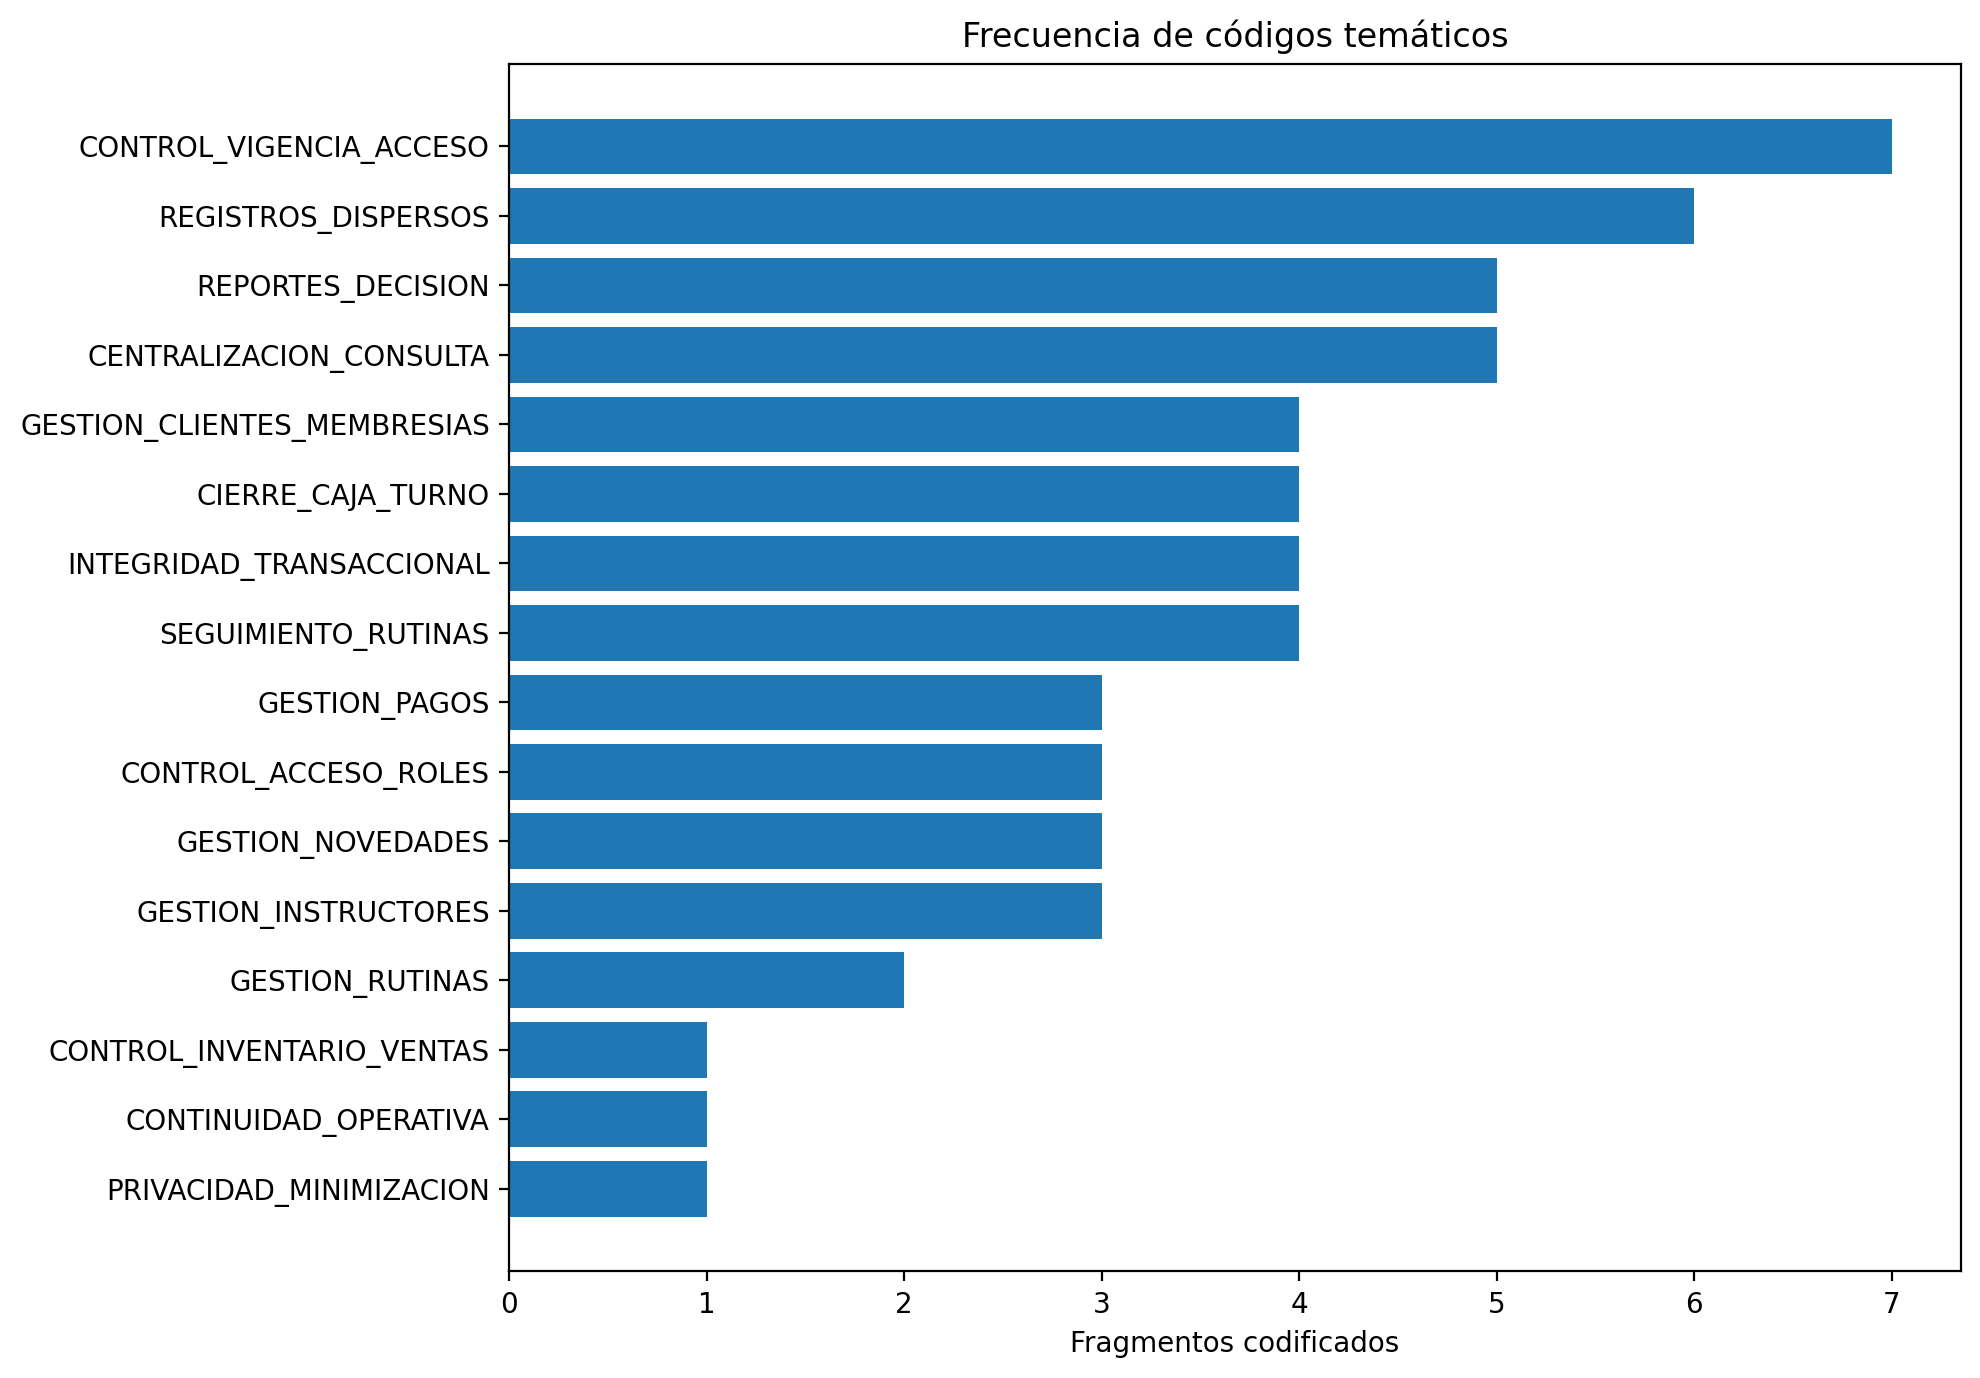
\includegraphics[width=0.88\textwidth]{figuras/frecuencias_codigos.png}
\caption{Frecuencia de códigos temáticos en los 59 fragmentos.}
\end{figure}

\begin{figure}[H]
\centering
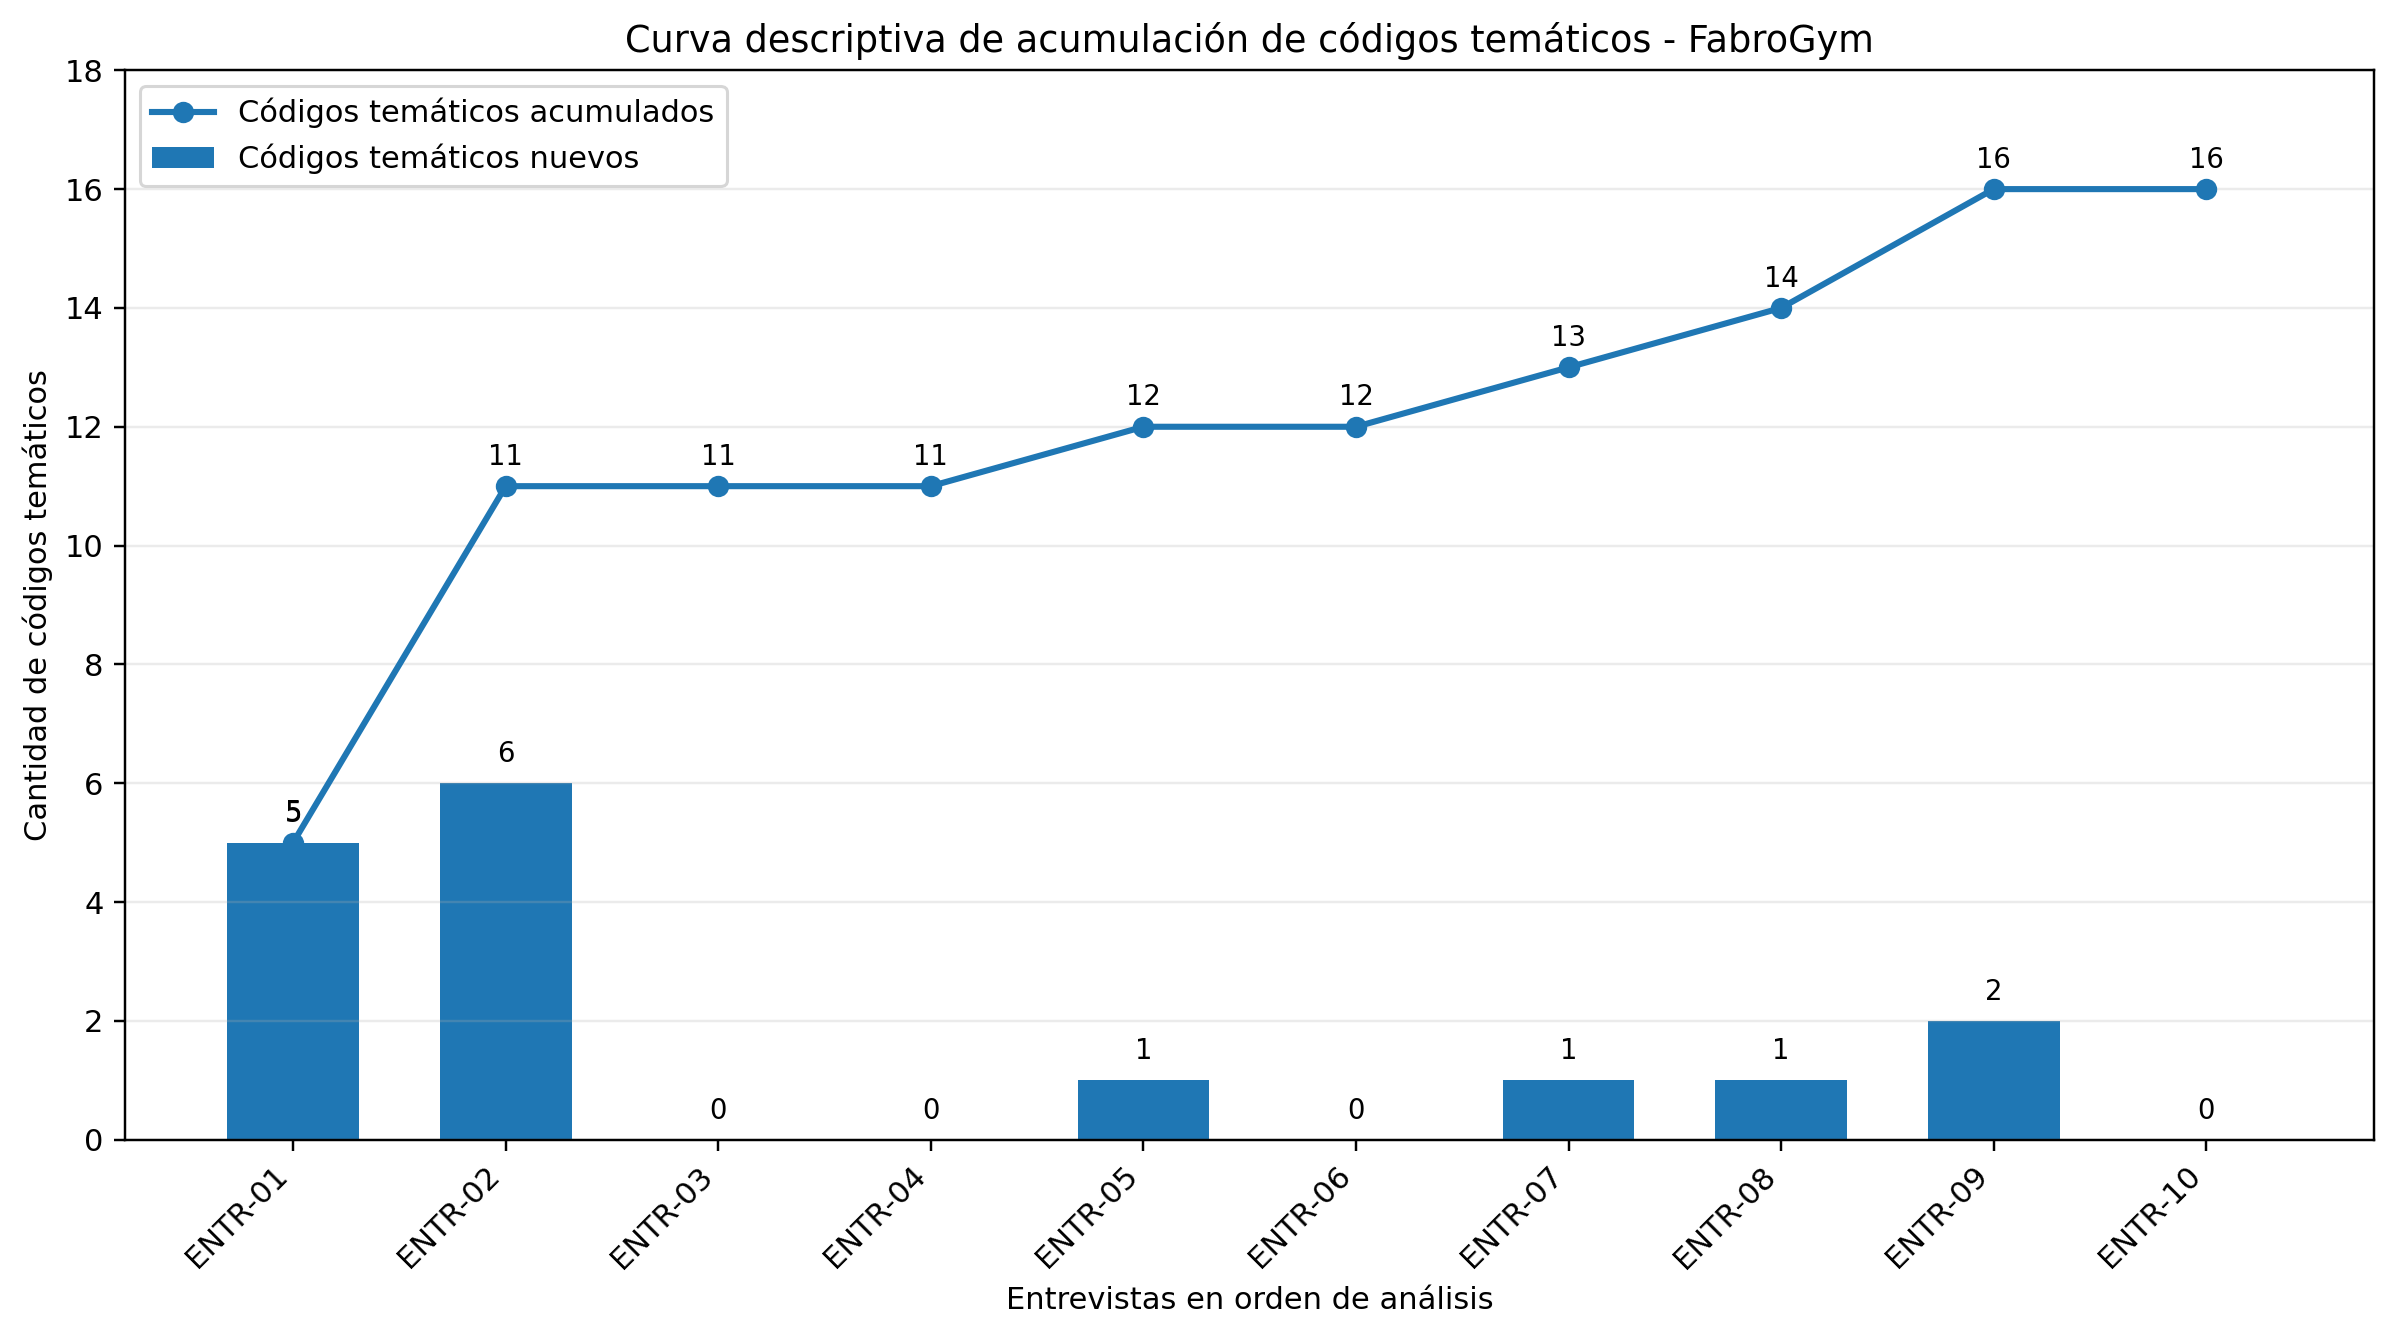
\includegraphics[width=0.88\textwidth]{figuras/curva_saturacion.png}
\caption{Curva descriptiva de códigos acumulados. No constituye demostración de saturación teórica.}
\end{figure}

\subsection{Análisis del cuestionario}

Se calcularon frecuencias y porcentajes por respuesta categórica. No se aplicaron pruebas inferenciales debido al tamaño, al muestreo no probabilístico y a la inclusión de registros de pilotaje. Los scripts reproducen las tablas y figuras desde el CSV abierto.

Como controles descriptivos, 18 de 32 personas (56.2\%) indicaron que consultan verbalmente en recepción el estado de la membresía; 16 (50.0\%) prefieren WhatsApp para avisos; 10 (31.2\%) priorizan mejorar las membresías; y 23 (71.9\%) consideran la privacidad importante o muy importante. Estos porcentajes describen exclusivamente la base observada.

\begin{figure}[H]
\centering
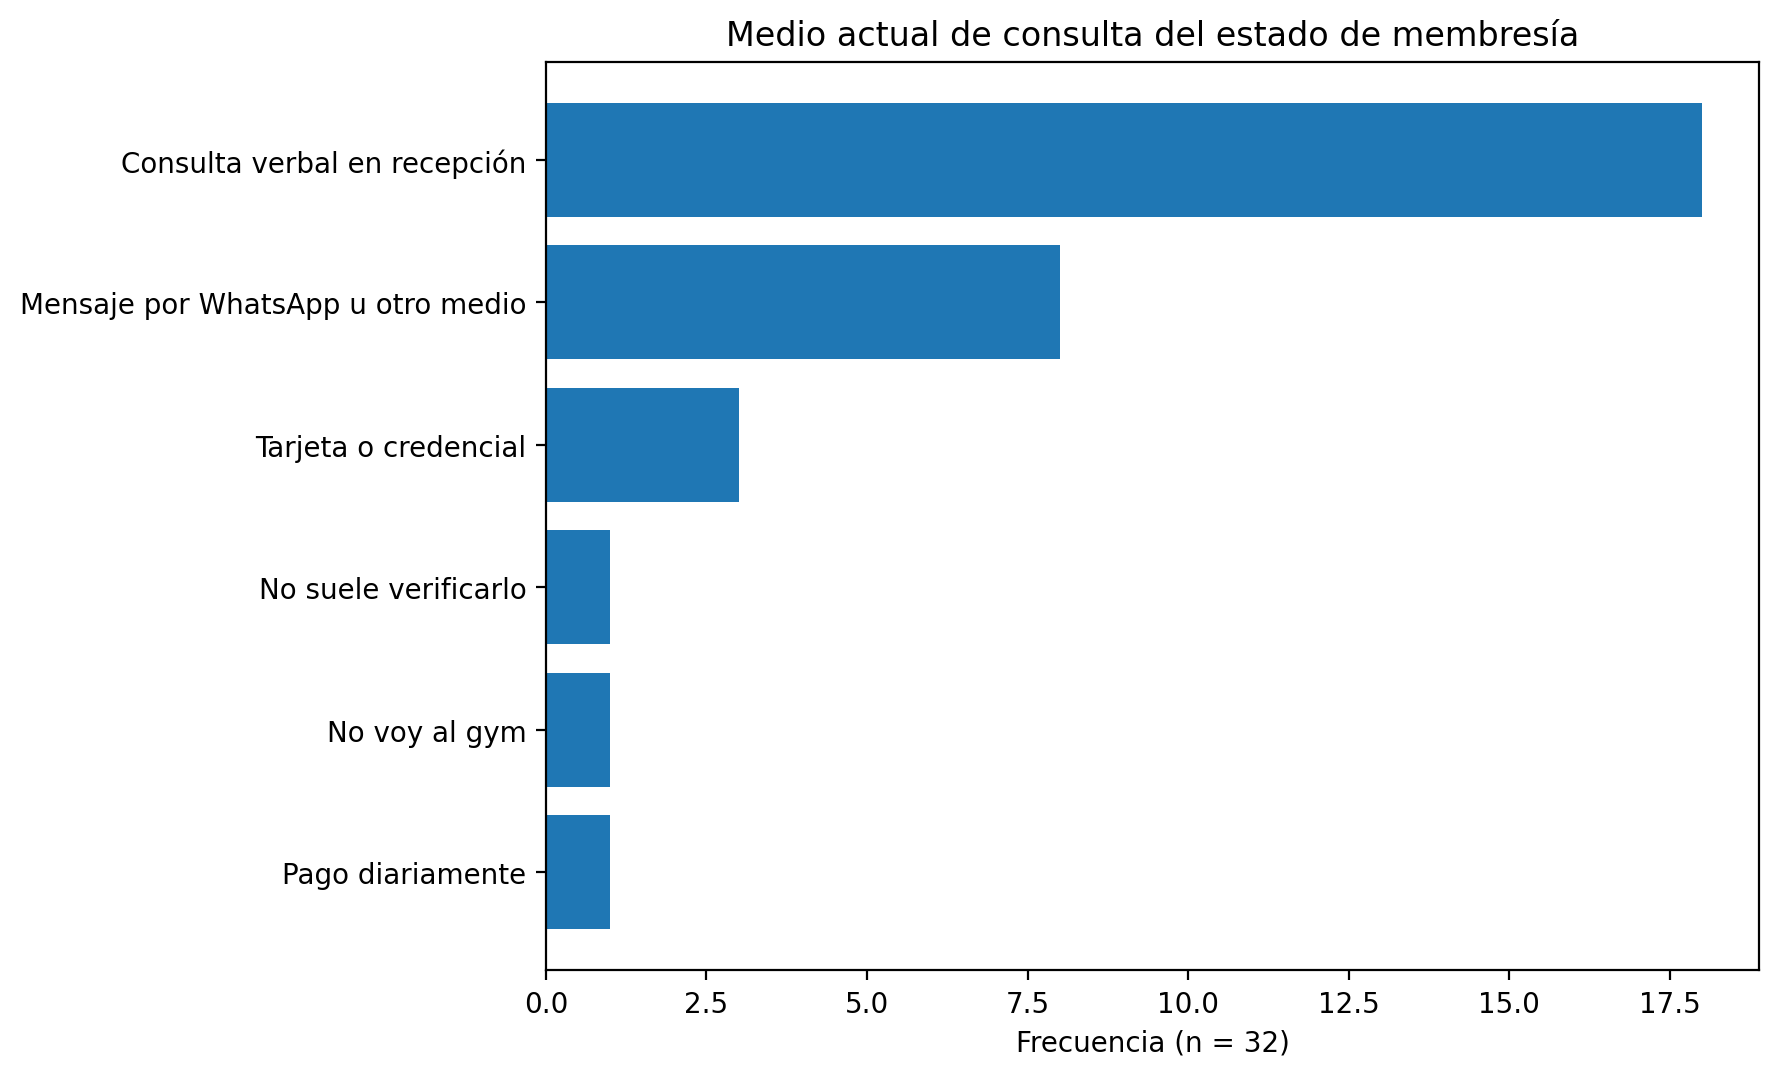
\includegraphics[width=0.86\textwidth]{figuras/consulta_membresia.png}
\caption{Medio actual de consulta del estado de membresía.}
\end{figure}

\begin{figure}[H]
\centering
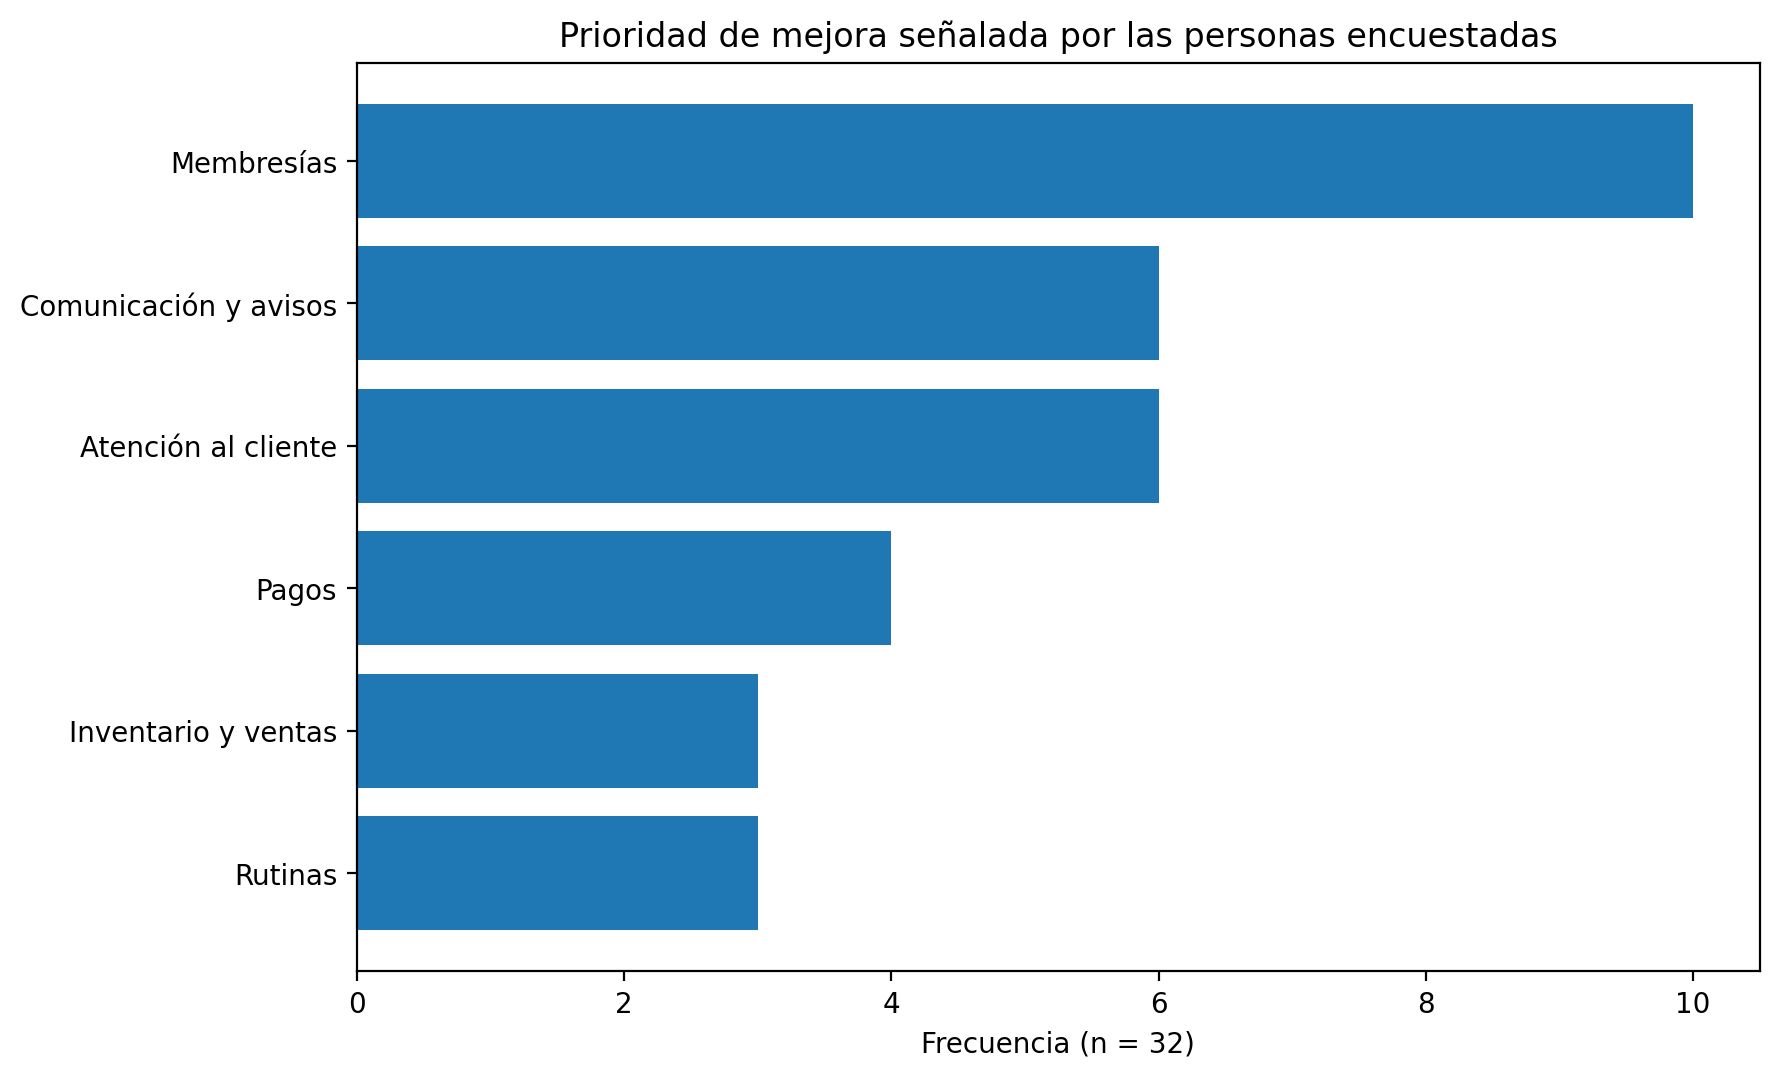
\includegraphics[width=0.86\textwidth]{figuras/prioridades_mejora.png}
\caption{Proceso señalado como primera prioridad de mejora.}
\end{figure}

\subsection{Derivación y trazabilidad}

Los fragmentos codificados se asociaron con candidatos a requisito. Cada requisito fue revisado y formalizado con identificador, descripción, fuente, stakeholder, prioridad y artefactos relacionados. Los RNF se cuantificaron conforme a ISO/IEC 25010:2023. Las restricciones legales y de diseño incluyen minimización, privacidad desde el diseño, derechos del titular y exclusión de IA sin una necesidad elicitada y una evaluación adicional.

La matriz sigue la cadena:
\[
\text{Fuente/Ley} \rightarrow \text{Objetivo} \rightarrow \text{Stakeholder} \rightarrow
\text{Evidencia} \rightarrow \text{RF/RNF/RD} \rightarrow \text{CU} \rightarrow
\text{HU} \rightarrow \text{CA} \rightarrow \text{Componente} \rightarrow \text{Mockup}.
\]

La depuración eliminó identificadores repetidos y dejó 44 elementos únicos. Los archivos CSV y JSON permiten verificar la correspondencia de forma automática.

\subsection{Ética y protección de datos}

La participación fue voluntaria. La publicación se limita a material anonimizado. Los archivos con datos identificables permanecen fuera del paquete abierto. Se aplicaron los siguientes principios:
\begin{enumerate}
\item minimización de datos;
\item seudonimización;
\item separación entre zona pública y restringida;
\item acceso limitado por finalidad;
\item exclusión de biometría y salud;
\item transparencia sobre pilotaje, muestra y actividades pendientes.
\end{enumerate}

\subsection{Reproducibilidad}

El paquete incluye CSV, JSON, diccionarios, figuras, licencia CC BY 4.0, archivo CITATION.cff y scripts en Python. Los scripts recalculan frecuencias, regeneran figuras y validan conteos, unicidad de identificadores y posibles secuencias de datos personales. El DOI no se incorpora hasta que Zenodo lo asigne.

\section{Resultados}
\pending. La Entrega 4 incorporará resultados integrados de RQ1--RQ3, validación walkthrough, cobertura funcional del MVP y análisis de defectos o cambios. En esta versión solo se reportan conteos y frecuencias descriptivas verificables.

\section{Discusión}
\pending. No se afirma que FabroGym mejore tiempos, errores o satisfacción hasta ejecutar pruebas y validaciones.

\section{Amenazas a la validez}
\pending. Las amenazas ya identificadas incluyen muestreo no probabilístico, cuatro respuestas de pilotaje, posible dependencia entre entrevistas, ausencia de saturación teórica demostrada, contexto local, codificación realizada por el equipo y validaciones pendientes.

\section{Conclusiones}
\pending. La conclusión final dependerá de la ejecución de la Entrega 4. La versión actual establece una base metodológica, trazable y reproducible sin atribuir efectos al sistema.

\bibliographystyle{IEEEtran}
\bibliography{referencias}

\end{document}
